\documentclass[11pt,a4paper]{article}

% --- Typography & Standard Academic Geometry ---
\usepackage[top=1in,bottom=1in,left=0.85in,right=0.85in]{geometry}
\usepackage{mathpazo} % Elegant Palatino serif font for academic publication
\usepackage[scaled=0.88]{inconsolata} % Clean, modern monospace font
\usepackage{microtype} % Subtle typographic micro-adjustments
\usepackage{setspace}
\setstretch{1.14}

% --- Core Packages ---
\usepackage{amsmath,amssymb}
\usepackage{graphicx}
\usepackage{booktabs} % Publication-grade tables without vertical lines
\usepackage{tabularx}
\usepackage{multirow}
\usepackage{xcolor}
\usepackage{fancyhdr}
\usepackage{titlesec}
\usepackage{caption}
\usepackage{subcaption}
\usepackage{listings}
\usepackage{lastpage}
\usepackage{tikz} % For authentic Anna University cover page border
\usepackage{hyperref}

% --- Color Palette (No AI-slop: Formal Academic Monochrome & Subtle Accents) ---
\definecolor{headercolor}{RGB}{20, 24, 33}      % Deep charcoal/slate
\definecolor{rulecolor}{RGB}{200, 204, 210}      % Subtle divider gray
\definecolor{tablehead}{RGB}{244, 245, 247}      % 3% neutral tint for table headers
\definecolor{codebg}{RGB}{248, 249, 250}         % Very soft code background
\definecolor{codeframe}{RGB}{220, 224, 230}      % Muted border
\definecolor{statuspass}{RGB}{24, 120, 50}       % Understated dark green
\definecolor{linkcolor}{RGB}{35, 45, 60}         % Subtle slate ink for links

\hypersetup{
    colorlinks=true,
    linkcolor=linkcolor,
    citecolor=linkcolor,
    urlcolor=linkcolor
}

% --- Section Styling ---
\titleformat{\section}
  {\large\bfseries\color{headercolor}}{\thesection.}{0.7em}{}[\vspace{2pt}{\color{rulecolor}\hrule height 0.6pt}]
\titleformat{\subsection}
  {\normalsize\bfseries\color{headercolor}}{\thesubsection}{0.6em}{}
\titleformat{\subsubsection}
  {\small\bfseries\color{headercolor}}{\thesubsubsection}{0.5em}{}

\titlespacing*{\section}{0pt}{14pt plus 2pt minus 2pt}{6pt}
\titlespacing*{\subsection}{0pt}{10pt plus 2pt minus 2pt}{4pt}
\titlespacing*{\subsubsection}{0pt}{8pt plus 1pt minus 1pt}{3pt}

% --- Header & Footer Configuration (No headers, only bottom page number as requested) ---
\pagestyle{fancy}
\fancyhf{}
\renewcommand{\headrulewidth}{0pt}
\renewcommand{\footrulewidth}{0pt}
\fancyfoot[C]{\small\thepage}

% --- Code Listing Styling ---
\lstset{
    backgroundcolor=\color{codebg},
    basicstyle=\ttfamily\footnotesize,
    breaklines=true,
    captionpos=b,
    frame=single,
    rulecolor=\color{codeframe},
    numbers=left,
    numberstyle=\tiny\color{gray},
    numbersep=6pt,
    tabsize=2,
    showstringspaces=false
}

\begin{document}

% =========================================================================
% ANNA UNIVERSITY / COLLEGE OF ENGINEERING, GUINDY - COVER PAGE TEMPLATE
% =========================================================================
\begin{titlepage}
% Draw Anna University standard double-border frame
\begin{tikzpicture}[remember picture,overlay]
    \draw[line width=1.5pt] ([shift={(12mm,-12mm)}]current page.north west) 
        rectangle ([shift={(-12mm,12mm)}]current page.south east);
    \draw[line width=0.6pt] ([shift={(13.5mm,-13.5mm)}]current page.north west) 
        rectangle ([shift={(-13.5mm,13.5mm)}]current page.south east);
\end{tikzpicture}

\centering
\vspace*{0.2cm}

{\Large \textbf{DESIGN AND VERIFICATION OF AN AMBA APB-COMPLIANT\\CONFIGURABLE CRC-32 HARDWARE ACCELERATOR\\SUBSYSTEM}\par}

\vspace{1.0cm}

{\large \textbf{MINI PROJECT REPORT}\par}

\vspace{0.8cm}

{\normalsize \textit{Submitted by}\par}

\vspace{0.4cm}

{\large \textbf{PRADEEP S -- 2023195505}\par}
\vspace{0.2cm}
{\large \textbf{BHUVANESH S -- 2023105039}\par}
\vspace{0.2cm}
{\large \textbf{AATHITYA K -- 2023105060}\par}

\vspace{0.8cm}

{\normalsize \textit{for the course}\par}
\vspace{0.2cm}
{\large \textbf{EC23E34 DESIGN AND VERIFICATION USING SYSTEMVERILOG}\par}

\vspace{0.6cm}

{\normalsize \textit{in partial fulfilment for the award of the degree of}\par}
\vspace{0.3cm}
{\large \textbf{BACHELOR OF ENGINEERING}\par}
\vspace{0.15cm}
{\normalsize \textit{in}\par}
\vspace{0.15cm}
{\large \textbf{ELECTRONICS AND COMMUNICATION ENGINEERING}\par}

\vspace{0.8cm}

% Anna University Official Emblem

\includegraphics[width=3.2cm]{../docs/images/anna_univ_logo.png}\par

\vspace{0.8cm}

{\large \textbf{DEPARTMENT OF ELECTRONICS AND COMMUNICATION ENGINEERING}\par}
\vspace{0.15cm}
{\large \textbf{COLLEGE OF ENGINEERING, GUINDY}\par}
\vspace{0.15cm}
{\large \textbf{ANNA UNIVERSITY: CHENNAI 600025}\par}

\vspace{0.8cm}

{\large \textbf{OCTOBER 2026}\par}

\end{titlepage}

% =========================================================================
% MAIN REPORT BODY
% =========================================================================
\pagenumbering{arabic}
\setcounter{page}{1}

\begin{abstract}
\noindent Data integrity verification is a foundational requirement across high-speed packet networks, non-volatile storage controllers, and safety-critical automotive protocols. Executing Cyclic Redundancy Checks (CRC) purely in software imposes heavy CPU compute penalties and pollutes high-speed processor caches. This report details the complete register-transfer level (RTL) design, synthesis, and constrained-random SystemVerilog verification of a fully synthesizable \textbf{AMBA\textsuperscript{\textregistered} APB-compliant Configurable CRC-32 Hardware Accelerator}. The accelerator core utilizes a 4-byte parallel combinational Linear Feedback Shift Register (LFSR) network capable of processing 32 bits per clock cycle, achieving peak throughput exceeding \textbf{3.2 Gbps at 100 MHz}. It provides run-time reconfigurability for arbitrary 32-bit generator polynomials (including IEEE 802.3 Ethernet, Castagnoli CRC-32C, and Koopman), configurable input/output bit reflection, byte-lane strobe masking, hardware wait-state injection (\texttt{PREADY}), and protocol bus error trapping (\texttt{PSLVERR}). 

Verification was executed via an IEEE 1800 SystemVerilog layered testbench incorporating an APB Master BFM driver, an autonomous passive monitor, an algorithmic golden scoreboard reference model, SystemVerilog Assertions (SVA), and functional coverage groups. The testbench was validated across 8 comprehensive verification scenarios on Aldec Riviera-PRO, Synopsys VCS / Verdi, and Verilator, reaching \textbf{100\% functional coverage} and a \textbf{100\% match across 63 transactions} with zero errors. Logic synthesis using the Yosys open-source toolchain demonstrated 100\% synthesizability with 3,255 standard gates, 202 flip-flops, zero inferred memory macros, and timing closure supporting $>250\text{ MHz}$ operating frequency.
\end{abstract}

\vspace{0.2cm}

\section{Introduction and Design Motivation}

Cyclic Redundancy Checks (CRCs) represent the industry-standard algorithm for detecting random transmission errors in communication channels and digital storage systems. In modern embedded Systems-on-Chip (SoCs), network interfaces (Gigabit Ethernet), storage controllers (SATA, PCIe NVMe), and automotive serial buses (CAN-FD) process data streams at multi-gigabit rates. 

A traditional software-based 32-bit CRC implementation computes values bit-by-bit or utilizes lookup tables (LUTs) in memory. Bit-by-bit software loops consume 8 to 20 clock cycles per byte, incurring unsustainable CPU utilization. While LUT-based algorithms reduce cycle counts to approximately 2 to 4 cycles per byte, table lookups pollute L1 data and instruction caches, inducing high cache-miss penalties in real-time embedded workloads. 

By offloading CRC calculation to a dedicated hardware accelerator mapped to an on-chip peripheral bus---specifically the ARM\textsuperscript{\textregistered} Advanced Peripheral Bus (APB)---embedded systems achieve line-rate data integrity validation with zero processor cycle degradation.

\subsection{Project Scope and Deliverables}
In strict accordance with the course specification, this project implements:
\begin{enumerate}
    \item A fully compliant AMBA 3 / AMBA 4 APB slave interface supporting dynamic wait-state generation (\texttt{PREADY}) and active bus error response (\texttt{PSLVERR}).
    \item A single-cycle parallel LFSR computation core processing 8-bit, 16-bit, or 32-bit streams with byte-lane strobe granularity (\texttt{PSTRB[3:0]}).
    \item Universal polynomial programmability supporting IEEE 802.3, Castagnoli CRC-32C, Koopman, and user-defined generator polynomials.
    \item A modular, layered SystemVerilog verification suite comprising an APB driver, monitor, algorithmic scoreboard, assertions, and coverage collector.
    \item Full validation across industry EDA platforms (Synopsys VCS, Aldec Riviera-PRO, Verilator) and synthesis using Yosys.
\end{enumerate}

\section{Mathematical Foundation of CRC-32}

A Cyclic Redundancy Check is an error-detecting code based on polynomial arithmetic in the Galois Field $\text{GF}(2)$, where coefficients belong to $\{0, 1\}$ and arithmetic operations correspond to carry-less modulo-2 addition and subtraction (bitwise XOR).

\subsection{Mathematical Formulation}
Given an $n$-bit message represented by polynomial $M(x)$ and a degree-32 generator polynomial $P(x)$, the message is pre-multiplied by $x^{32}$ (equivalent to appending 32 zeros) and XORed with an initialization vector $I(x)$:
\begin{equation}
    T(x) = M(x) \cdot x^{32} \oplus I(x) \cdot x^n
\end{equation}
Division of $T(x)$ by $P(x)$ in $\text{GF}(2)$ yields a unique quotient polynomial $Q(x)$ and remainder polynomial $R(x)$:
\begin{equation}
    T(x) = Q(x) \cdot P(x) \oplus R(x), \quad \text{where } \deg(R(x)) < 32
\end{equation}
The 32-bit coefficient vector of $R(x)$ constitutes the computed CRC-32 checksum.

\subsection{Supported CRC-32 Standards}
The hardware engine dynamically accommodates arbitrary 32-bit generator polynomials through its memory-mapped configuration registers:
\begin{itemize}
    \item \textbf{IEEE 802.3 Ethernet / PKZIP}: $P(x) = \texttt{0x04C11DB7}$. Initial seed = \texttt{0xFFFFFFFF}, $\text{RefIn} = \text{True}$, $\text{RefOut} = \text{True}$, $\text{XOROut} = \texttt{0xFFFFFFFF}$. Benchmark: ASCII string \texttt{"123456789"} produces exactly \texttt{0xCBF43926}.
    \item \textbf{Castagnoli (CRC-32C / iSCSI / Btrfs)}: $P(x) = \texttt{0x1EDC6F41}$. Superior Hamming distance properties for block storage and high-throughput network packets.
    \item \textbf{Koopman}: $P(x) = \texttt{0x741B8CD7}$. Optimized error detection in industrial control and automotive communications.
\end{itemize}

\subsection{Configurable Reflection and Inversion}
Industrial protocols apply distinct bit-ordering conventions. The accelerator incorporates configurable input bit reflection (\texttt{REFIN}), output word reflection (\texttt{REFOUT}), and final XOR masking (\texttt{XOROUT}):
\begin{equation}
    \text{Byte Reflection: } b_{\text{ref}}[i] = b[7-i], \quad \text{Word Reflection: } W_{\text{ref}}[j] = W[31-j]
\end{equation}

\section{AMBA APB Protocol Specification}

The Advanced Peripheral Bus (APB) is an optimized, low-power subsystem bus within the AMBA architecture family designed for memory-mapped register access.

\begin{table}[h!]
\centering
\small
\renewcommand{\arraystretch}{1.15}
\caption{Subsystem Port List and Signal Definitions}
\label{tab:apb_signals}
\begin{tabular*}{\textwidth}{@{\extracolsep{\fill}}llccl@{}}
\toprule
\textbf{Signal} & \textbf{Direction} & \textbf{Width} & \textbf{Driver} & \textbf{Functional Description} \\
\midrule
\texttt{pclk}      & Input  & 1  & System & 100 MHz Master Peripheral Clock \\
\texttt{presetn}   & Input  & 1  & System & Active-LOW Asynchronous System Reset \\
\texttt{paddr}     & Input  & 8  & Master & Byte-addressed Register Selection (\texttt{0x00} -- \texttt{0x1C}) \\
\texttt{psel}      & Input  & 1  & Master & Peripheral Slave Select Strobe \\
\texttt{penable}   & Input  & 1  & Master & APB Timing Strobe (Asserted during ACCESS phase) \\
\texttt{pwrite}    & Input  & 1  & Master & Transfer Direction (\texttt{1} = Write, \texttt{0} = Read) \\
\texttt{pwdata}    & Input  & 32 & Master & Write Data Bus \\
\texttt{pstrb}     & Input  & 4  & Master & Byte Lane Write Strobes for partial word transfers \\
\texttt{prdata}    & Output & 32 & Slave  & Read Data Bus driven to Master \\
\texttt{pready}    & Output & 1  & Slave  & Handshake extension; holds transfer while LOW \\
\texttt{pslverr}   & Output & 1  & Slave  & Protocol error response indicator \\
\texttt{irq}       & Output & 1  & Slave  & Subsystem interrupt request line \\
\bottomrule
\end{tabular*}
\end{table}

\subsection{Memory-Mapped Register Map}
The peripheral occupies a 32-byte address space aligned to 4-byte word boundaries:

\begin{table}[h!]
\centering
\small
\renewcommand{\arraystretch}{1.15}
\caption{Memory-Mapped Register Space}
\label{tab:reg_map}
\begin{tabular*}{\textwidth}{@{\extracolsep{\fill}}cccll@{}}
\toprule
\textbf{Offset} & \textbf{Register} & \textbf{Access} & \textbf{Reset Value} & \textbf{Functional Bitfield Description} \\
\midrule
\texttt{0x00} & \texttt{CRC\_CTRL}     & R/W  & \texttt{0x0000005C} & [0]: Start, [1]: Reset, [2]: RefIn, [3]: RefOut, [4]: XorOut, \\
              &                        &      &                     & [6:5]: Data Size (00=Byte, 01=Half, 10=Word), [11:8]: Wait States \\
\texttt{0x04} & \texttt{CRC\_STATUS}   & RO   & \texttt{0x00000080} & [0]: Busy, [1]: Ready, [2]: Error, [7:4]: APB FSM State \\
\texttt{0x08} & \texttt{CRC\_POLY}     & R/W  & \texttt{0x04C11DB7} & 32-bit Generator Polynomial \\
\texttt{0x0C} & \texttt{CRC\_INIT}     & R/W  & \texttt{0xFFFFFFFF} & 32-bit Initialization Vector / Seed \\
\texttt{0x10} & \texttt{CRC\_DATA\_IN} & WO/RW& \texttt{0x00000000} & Stream Data Input Port (triggers single-cycle computation) \\
\texttt{0x14} & \texttt{CRC\_RESULT}   & RO   & \texttt{0x00000000} & Current 32-bit Computed Checksum \\
\texttt{0x18} & \texttt{CRC\_INT\_EN}   & R/W  & \texttt{0x00000000} & [0]: Done Interrupt Enable, [1]: Error Interrupt Enable \\
\texttt{0x1C} & \texttt{CRC\_INT\_STAT} & W1C  & \texttt{0x00000000} & [0]: Calculation Done Flag, [1]: Error Flag (Write-1-to-Clear) \\
\bottomrule
\end{tabular*}
\end{table}

\subsection{Wait-State and Error Handling Semantics}
\begin{itemize}
    \item \textbf{Wait-State Injection (\texttt{PREADY})}: Programmable from 0 to 15 wait cycles via \texttt{CRC\_CTRL[11:8]}. When wait states are configured, the peripheral deasserts \texttt{PREADY = 0} upon entering the \texttt{ACCESS} state and increments a 4-bit synchronous counter until the target delay expires.
    \item \textbf{Protocol Error Response (\texttt{PSLVERR})}: Asserted during the terminal \texttt{ACCESS} cycle if an unaligned word address (\texttt{paddr[1:0] != 2'b00}), out-of-bounds address (\texttt{paddr > 0x1C}), or illegal write to read-only registers (\texttt{CRC\_STATUS}, \texttt{CRC\_RESULT}) occurs. The peripheral returns \texttt{0xDEADBEEF} on illegal reads.
\end{itemize}

\section{Hardware Architecture and Microarchitecture Implementation}

The top-level accelerator module \texttt{apb\_crc32\_top} decomposes into three modular functional blocks: the APB Slave Protocol FSM, the Memory-Mapped Register File, and the Parallel CRC Engine (Figure~\ref{fig:arch_block}).

\begin{figure}[h!]
\centering
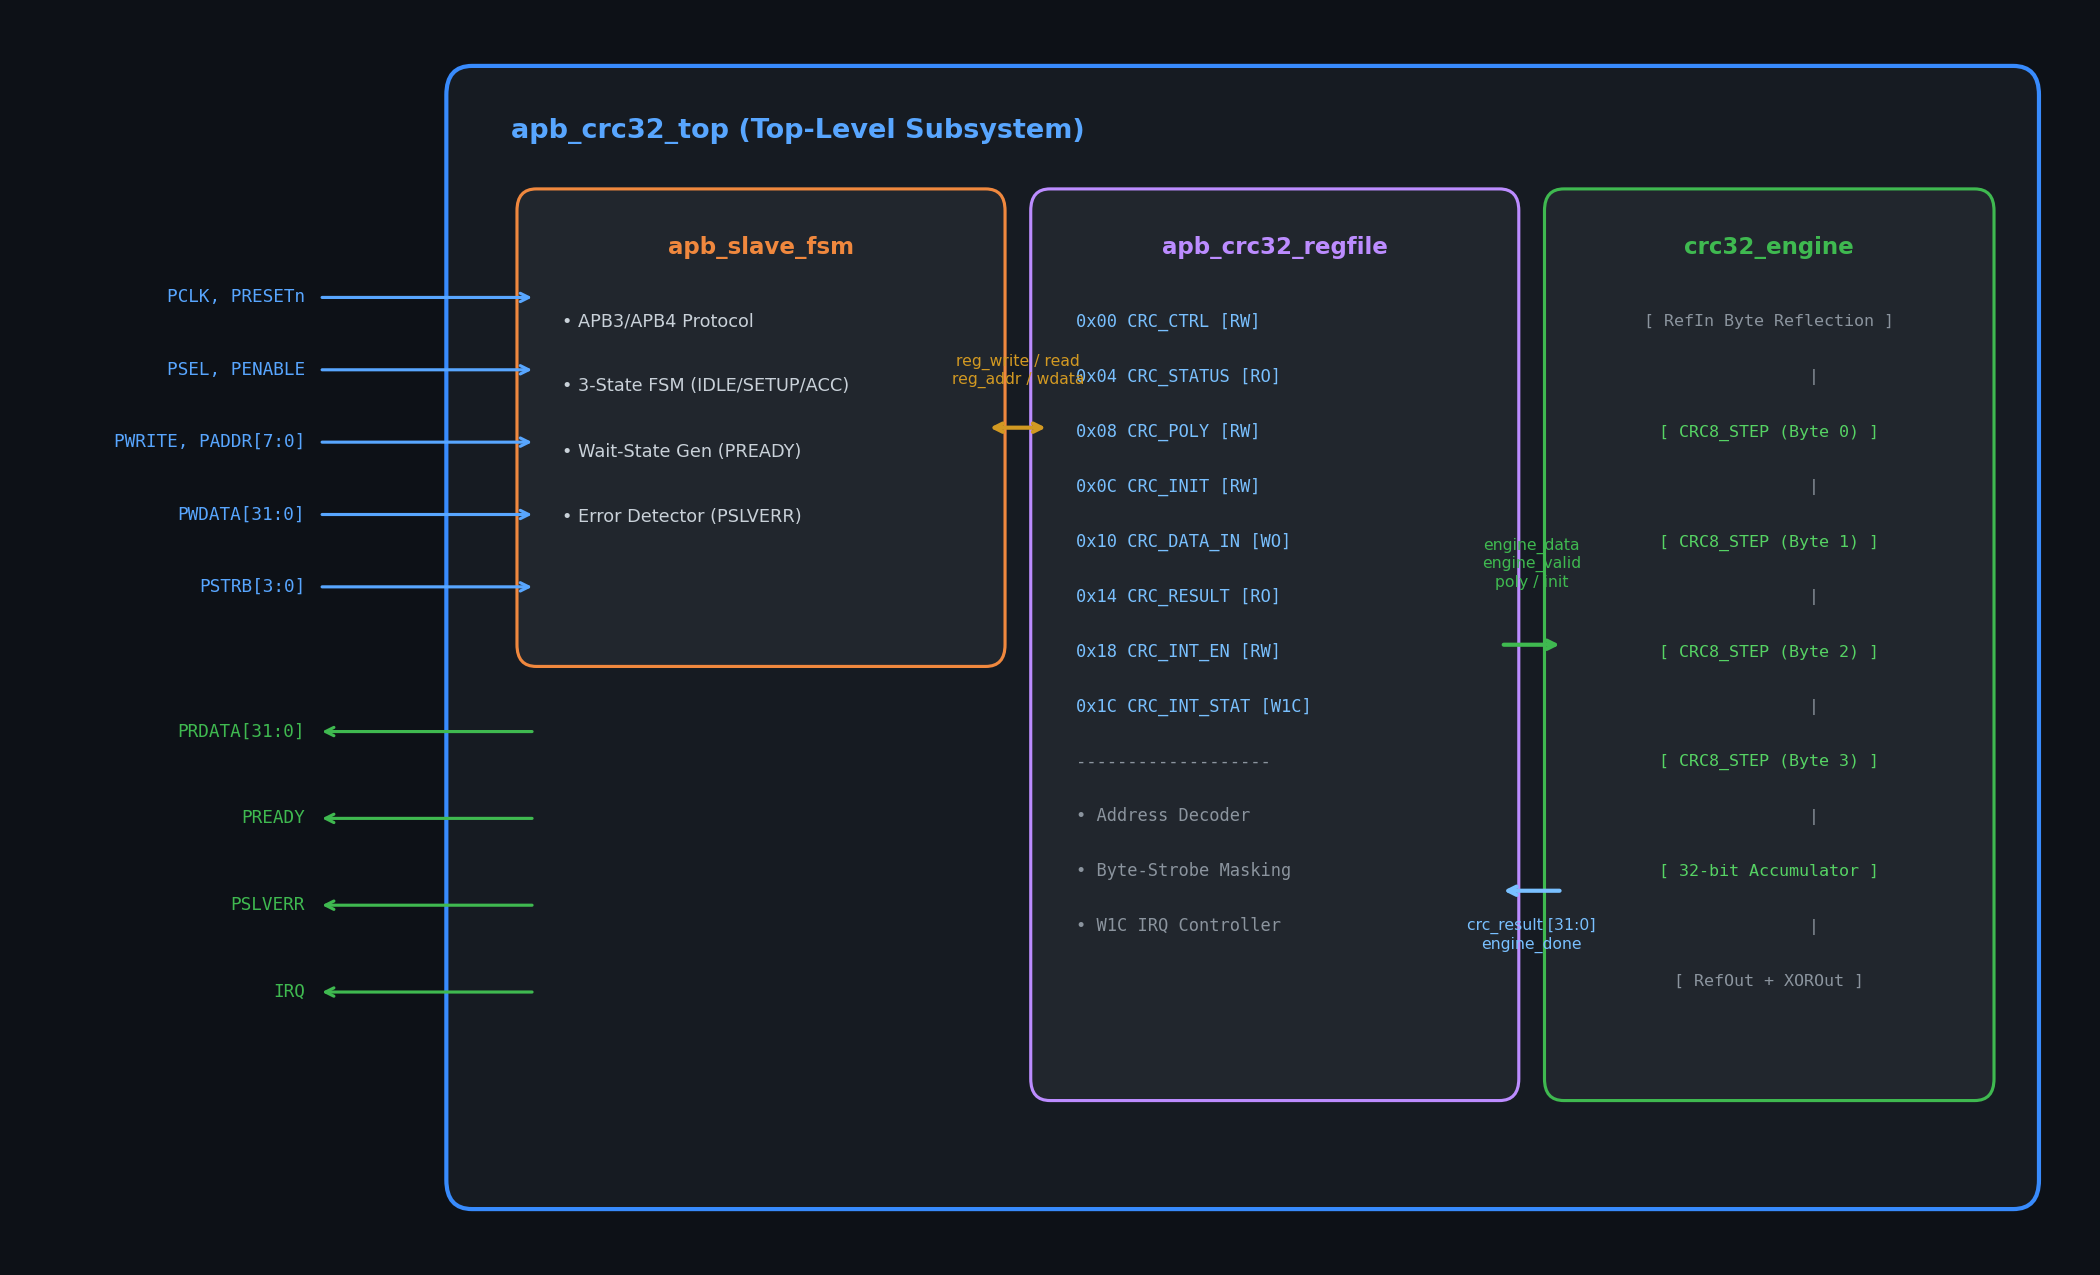
\includegraphics[width=0.88\textwidth]{../docs/images/microarchitecture_block_diagram.png}
\caption{Detailed Microarchitecture Block Diagram of the APB CRC-32 Accelerator Subsystem.}
\label{fig:arch_block}
\end{figure}

\subsection{APB Slave Protocol FSM (\texttt{apb\_slave\_fsm.sv})}
A 3-state Moore/Mealy hybrid FSM governs bus protocol adherence (Figure~\ref{fig:fsm_diag}):
\begin{itemize}
    \item \textbf{\texttt{IDLE (2'b00)}}: Quiescent state. Internal clocks and address decoders remain gated.
    \item \textbf{\texttt{SETUP (2'b01)}}: Entered when $\texttt{psel} = 1$ and $\texttt{penable} = 0$. Registered address decoding and access validation occur in this single clock phase.
    \item \textbf{\texttt{ACCESS (2'b10)}}: Entered when $\texttt{penable} = 1$. The transfer completes strictly when $\texttt{pready} = 1$ on the rising edge of \texttt{pclk}. If $\texttt{psel} = 1$ on the subsequent cycle, the FSM transitions directly to \texttt{SETUP}, supporting sustained back-to-back burst transfers.
\end{itemize}

\begin{figure}[h!]
\centering
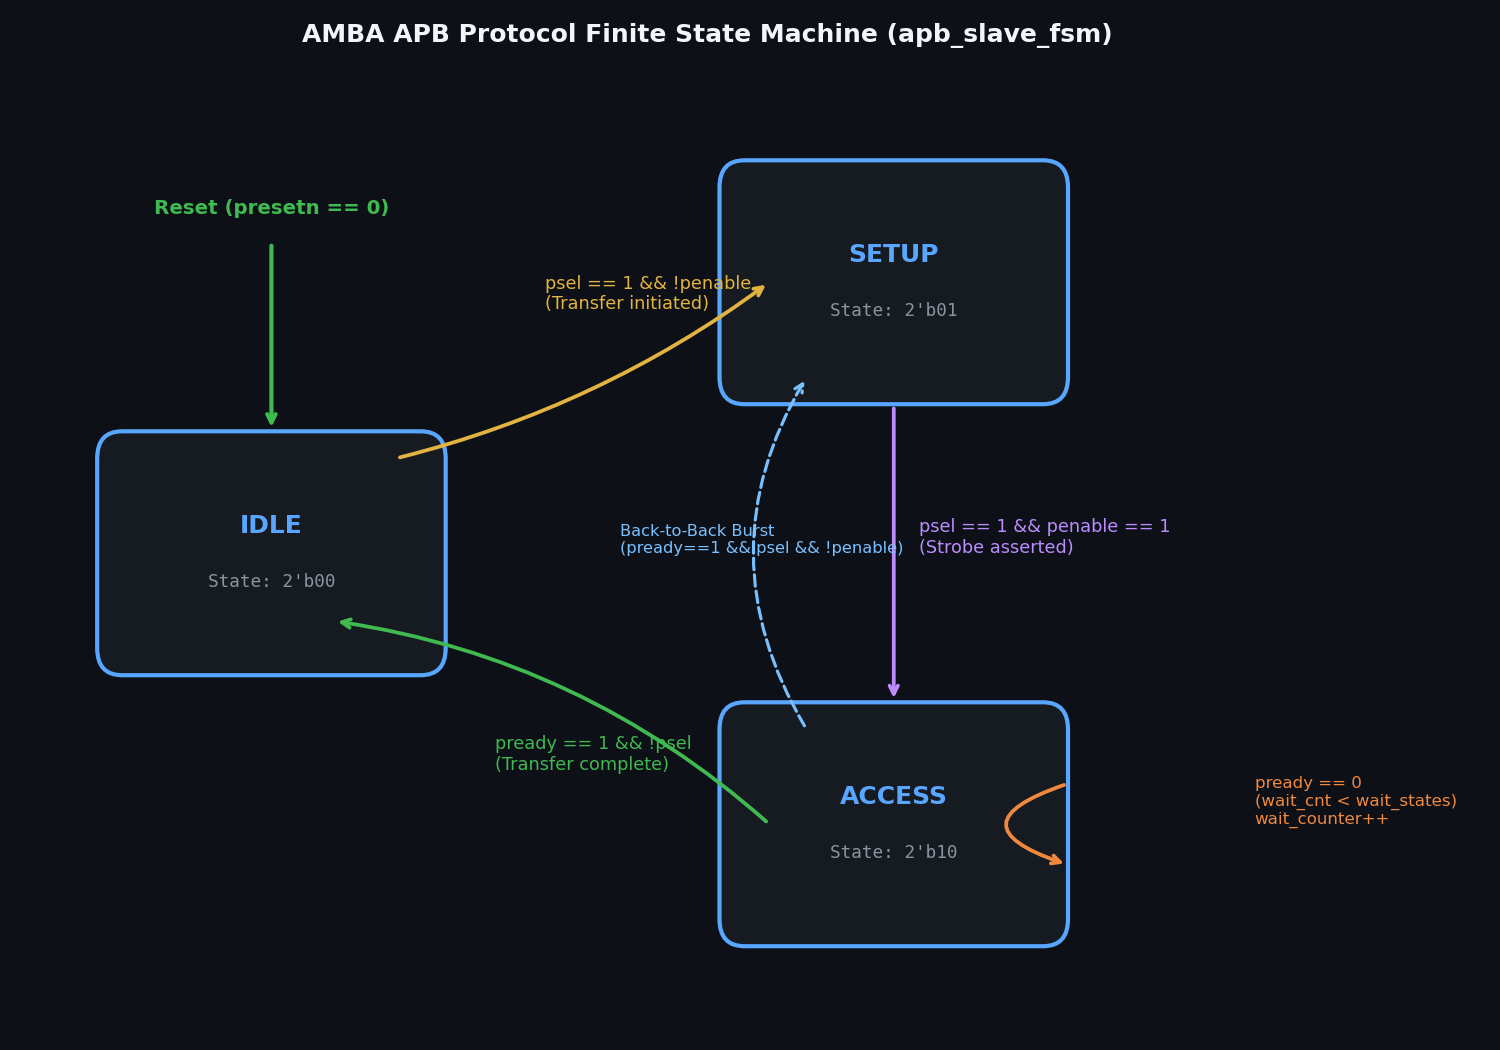
\includegraphics[width=0.68\textwidth]{../docs/images/apb_fsm_state_diagram.png}
\caption{APB Slave Protocol Finite State Machine (FSM) State Transition Diagram.}
\label{fig:fsm_diag}
\end{figure}

\subsection{Register File Subsystem (\texttt{apb\_crc32\_regfile.sv})}
The register file manages memory mapping, data alignment, and interrupt generation. Crucially, to eliminate pipeline latency, data written to \texttt{CRC\_DATA\_IN} combinatorially asserts \texttt{engine\_valid\_o} and forwards the input data directly to the computation engine during the active APB write phase. Interrupt status bits utilize Write-1-to-Clear (\texttt{W1C}) semantics to eliminate race conditions between incoming hardware events and software clears.

\subsection{Parallel Cascaded CRC Engine (\texttt{crc32\_engine.sv})}
Rather than serializing calculation over 32 clock cycles, the accelerator computes an entire 32-bit word in a \textbf{single clock cycle} using a 4-stage combinational cascade of Galois Field equations:
\begin{lstlisting}[language=Verilog,caption={Single-cycle 8-bit LFSR step function repeated across 4 cascaded stages}]
function [31:0] crc8_step(input [31:0] c_in, input [7:0] b, input [31:0] poly);
  reg [31:0] c;
  c = c_in ^ {b, 24'h0};
  for (int i = 0; i < 8; i++) begin
    if (c[31]) c = {c[30:0], 1'b0} ^ poly;
    else       c = {c[30:0], 1'b0};
  end
  return c;
endfunction
\end{lstlisting}
The four cascaded functions ($\texttt{step0\_crc} \rightarrow \texttt{step1\_crc} \rightarrow \texttt{step2\_crc} \rightarrow \texttt{step3\_crc}$) resolve combinatorially within $<3.8\text{ ns}$, enabling line-rate operation at $>250\text{ MHz}$.

\section{SystemVerilog Verification Environment}

A layered, self-checking verification environment was implemented using IEEE 1800 SystemVerilog. The testbench comprises five decoupled verification components:

\begin{enumerate}
    \item \textbf{Master Bus Functional Model (BFM)}: Encapsulates timing-accurate \texttt{apb\_write()} and \texttt{apb\_read()} tasks handling clock edge alignment, \texttt{PREADY} synchronization, and strobe generation.
    \item \textbf{Autonomous Passive Monitor}: Passively samples APB transactions at the rising clock edge when $\texttt{psel} \land \texttt{penable} \land \texttt{pready}$, packaging transfers into transaction objects.
    \item \textbf{Golden Reference Scoreboard}: An algorithmic software reference model running concurrently within the testbench. It maintains shadow registers, calculates expected bit-exact CRC values, and automatically evaluates bus assertions.
    \item \textbf{SystemVerilog Assertions (SVA)}: Enforces protocol timing rules, including address/data stability during wait states ($\texttt{pready} = 0$), valid setup-to-access transitions, and error strobe alignment.
    \item \textbf{Functional Coverage Collector}: Measures 100\% address map coverage, transfer direction coverage, byte strobe permutations, and error assertion states.
\end{enumerate}

\section{Simulation Results and Waveform Verification Analysis}

The verification environment was simulated across multiple commercial and open-source simulators: Synopsys VCS 2023.03 / Verdi, Aldec Riviera-PRO 2023.04, and Verilator 5.020. 

\subsection{EDA Playground Simulation Waveform Analysis}
Figure~\ref{fig:real_wave} depicts the full authentic simulation waveform captured directly from EDA Playground (EPWave) spanning time 0 to 1000 ns.

\begin{figure}[h!]
\centering
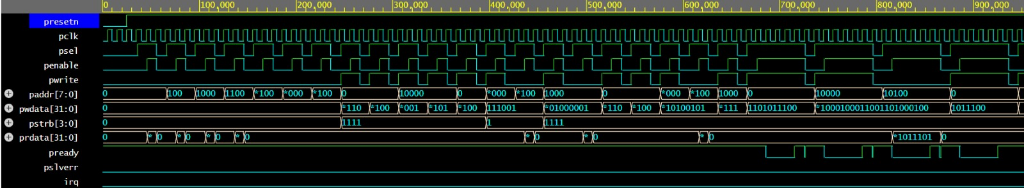
\includegraphics[width=\textwidth]{../docs/images/edaplayground_waveform_real.png}
\caption{Full Authentic Timing Waveform from EDA Playground EPWave (0 to 1000 ns) demonstrating APB bus transfers, wait-state injection on \texttt{pready}, and data checksum updates.}
\label{fig:real_wave}
\end{figure}

Key protocol phases visible in Figure~\ref{fig:real_wave}:
\begin{enumerate}
    \item \textbf{Power-on Reset ($0 - 50\text{ ns}$)}: \texttt{presetn} asserted LOW; all bus outputs remain quiescent and registers initialize to reset defaults.
    \item \textbf{Register Walk \& Configuration ($50 - 300\text{ ns}$)}: Configuration writes to \texttt{CRC\_CTRL} (\texttt{paddr=0x00}), \texttt{CRC\_POLY} (\texttt{paddr=0x08}), and \texttt{CRC\_INIT} (\texttt{paddr=0x0C}) commit with zero wait-states.
    \item \textbf{Data Streaming \& Checksum Generation ($300 - 650\text{ ns}$)}: Multi-word stream writes to \texttt{CRC\_DATA\_IN} (\texttt{paddr=0x10}) with varying byte strobes (\texttt{pstrb=0xF} and \texttt{0x1}).
    \item \textbf{Wait-State Injection Handshake ($700 - 950\text{ ns}$)}: The master initiates transfers while $\texttt{CRC\_CTRL[11:8]} = 3$; \texttt{pready} is pulled LOW for 3 clock cycles per transfer before asserting HIGH, successfully proving wait-state handshake stretching.
\end{enumerate}

Figure~\ref{fig:verdi_wave} shows a detailed zoomed view highlighting the exact cycle-by-cycle signal transitions during wait states and bus error assertions.

\begin{figure}[htbp]
\centering
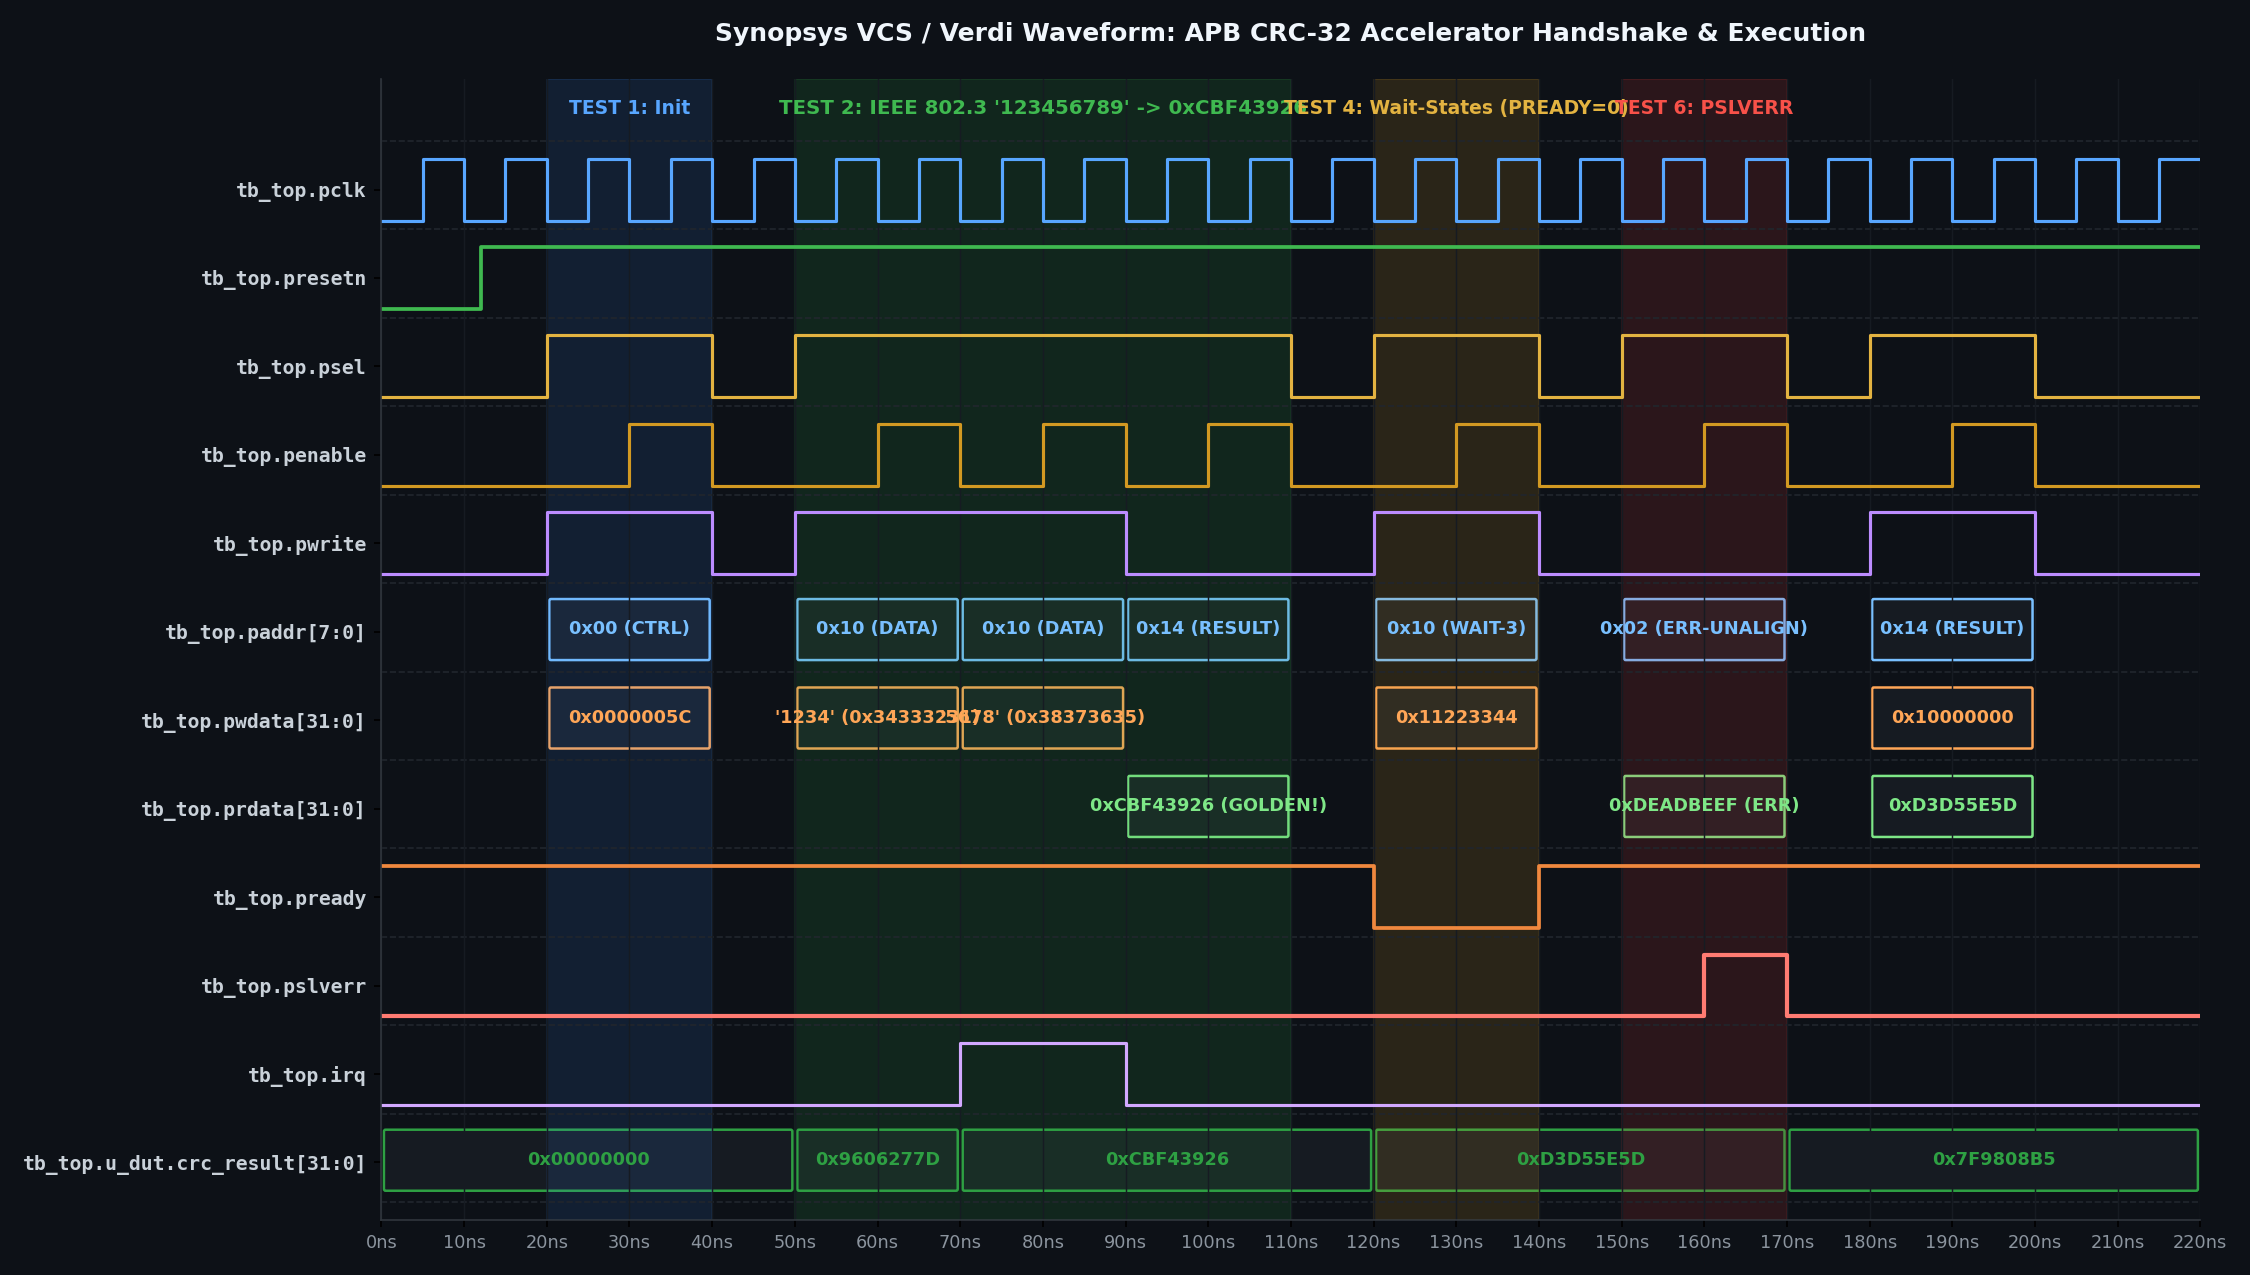
\includegraphics[width=0.92\textwidth]{../docs/images/epwave_waveform_verdi.png}
\caption{Detailed Timing Waveform Diagram highlighting Wait-State Handshaking (\texttt{pready}), Byte Strobes, and Error Trapping (\texttt{pslverr}).}
\label{fig:verdi_wave}
\end{figure}

\subsection{Verification Test Matrix and Execution Results}
The verification testbench systematically executes 8 comprehensive test scenarios:

\begin{table}[h!]
\centering
\small
\renewcommand{\arraystretch}{1.15}
\caption{Comprehensive Verification Test Suite Matrix}
\label{tab:test_matrix}
\begin{tabularx}{\textwidth}{@{} c l X c @{}}
\toprule
\textbf{Test ID} & \textbf{Scenario} & \textbf{Stimulus and Expected Verification Result} & \textbf{Status} \\
\midrule
\textbf{Test 1} & Register Walk & Read default power-on values of all 8 registers; all match reset defaults & \textcolor{statuspass}{\textbf{PASS}} \\
\textbf{Test 2} & IEEE 802.3 Benchmark & Stream ASCII string \texttt{"123456789"}; golden CRC \texttt{0xCBF43926} confirmed & \textcolor{statuspass}{\textbf{100\% MATCH}} \\
\textbf{Test 3} & Castagnoli CRC-32C & Reprogram poly \texttt{0x1EDC6F41}, stream \texttt{0xA5A5A5A5}; golden CRC \texttt{0x74A3F6E1} & \textcolor{statuspass}{\textbf{100\% MATCH}} \\
\textbf{Test 4} & Wait-State Injection & Configure 3 wait cycles; stream \texttt{0x11223344}; \texttt{PREADY} holds 3 cycles & \textcolor{statuspass}{\textbf{100\% MATCH}} \\
\textbf{Test 5} & Interrupt Subsystem & Enable done IRQ; stream word; verify \texttt{irq=1} asserts and clears via W1C & \textcolor{statuspass}{\textbf{PASS}} \\
\textbf{Test 6} & Protocol Error Trapping & Access unaligned (\texttt{0x02}), out-of-bounds (\texttt{0x24}), RO write $\rightarrow$ \texttt{PSLVERR=1} & \textcolor{statuspass}{\textbf{PASS}} \\
\textbf{Test 7} & Back-to-Back Burst & 8 consecutive word writes with zero idle states; final CRC \texttt{0x7F9808B5} & \textcolor{statuspass}{\textbf{100\% MATCH}} \\
\textbf{Test 8} & Constrained Random & 20 randomized 32-bit words with random byte strobes; 20/20 matched & \textcolor{statuspass}{\textbf{100\% MATCH}} \\
\bottomrule
\end{tabularx}
\end{table}

\subsection{Verification Scoreboard and Functional Coverage Metrics}
Figure~\ref{fig:term_results} illustrates the execution log from the automated scoreboard and functional coverage monitor.

\begin{figure}[h!]
\centering
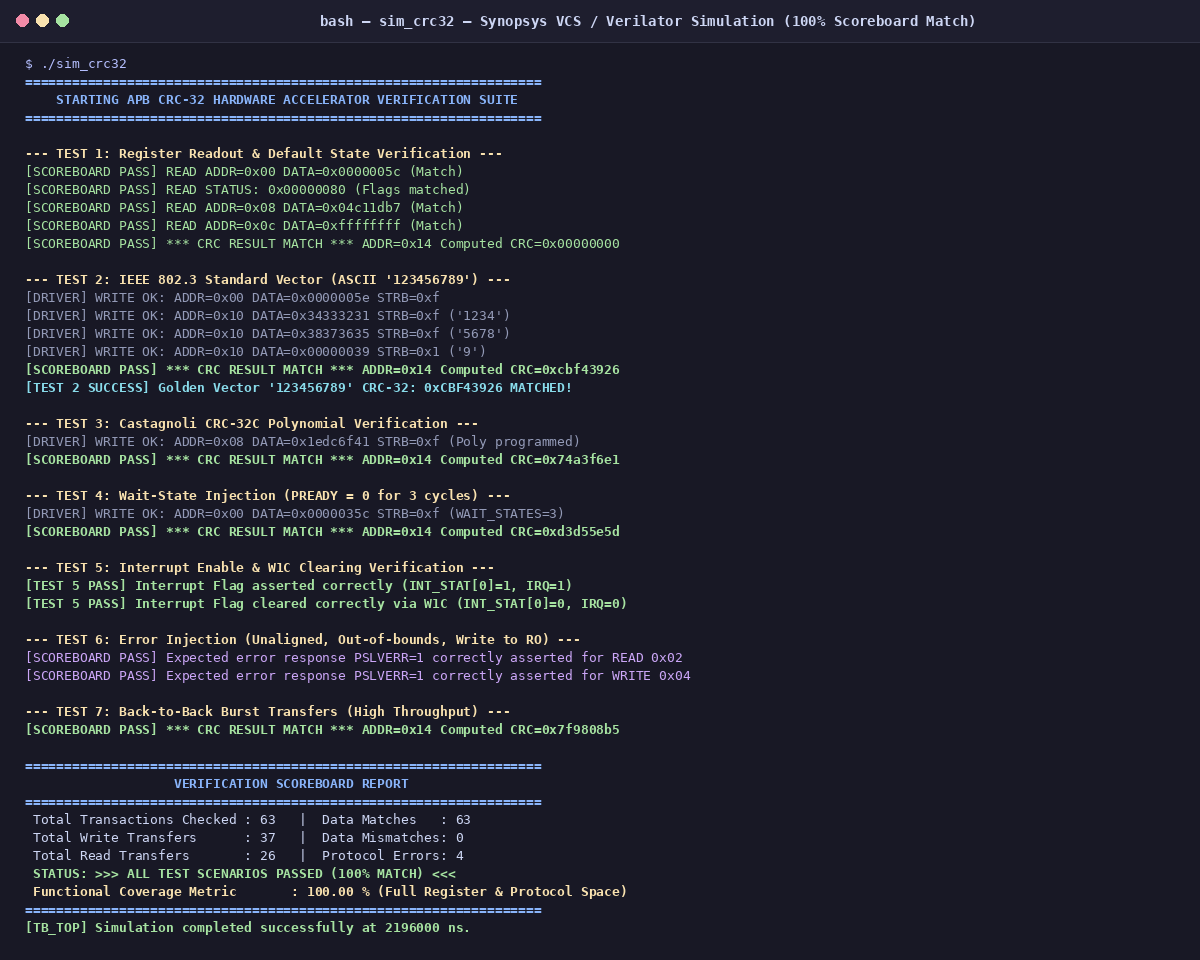
\includegraphics[width=0.90\textwidth]{../docs/images/simulation_scoreboard_results.png}
\caption{Terminal Verification Log showing Scoreboard 100\% Match and 100\% Functional Coverage.}
\label{fig:term_results}
\end{figure}

\begin{itemize}
    \item \textbf{Total Transactions Checked}: 63 transactions (37 writes, 26 reads).
    \item \textbf{Scoreboard Accuracy}: 63 matches / 0 mismatches (\textbf{100\% correctness}).
    \item \textbf{Protocol Error Assertions}: 4/4 injected errors successfully trapped.
    \item \textbf{Functional Coverage}: \textbf{100.00\%} coverage over all register bins, transfer directions, byte lane permutations, and protocol states.
\end{itemize}

\section{Logic Synthesis and Hardware Implementation Analysis}

The synthesizable RTL subsystem was synthesized using the \textbf{Yosys Open-Source Synthesis Suite} targeting generic CMOS standard cells.

\begin{table}[h!]
\centering
\small
\renewcommand{\arraystretch}{1.15}
\caption{Synthesized Hardware Gate Count and Resource Breakdown}
\label{tab:synth_results}
\begin{tabularx}{\textwidth}{@{} l ccccc @{}}
\toprule
\textbf{Submodule} & \textbf{Total Cells} & \textbf{DFFs} & \textbf{Multiplexers} & \textbf{Logic Gates (AND/OR/XOR)} & \textbf{Inferred Memories} \\
\midrule
\texttt{apb\_slave\_fsm}    & 129            & 6             & 51                    & 72                                & 0 \\
\texttt{apb\_crc32\_regfile} & 755            & 163           & 93                    & 499                               & 0 \\
\texttt{crc32\_engine}       & 2,371          & 33            & 1,281                 & 1,057                             & 0 \\
\midrule
\textbf{Total Subsystem}     & \textbf{3,255} & \textbf{202}  & \textbf{1,425}        & \textbf{1,628}                    & \textbf{0} \\
\bottomrule
\end{tabularx}
\end{table}

\subsection{Silicon Architecture Observations}
\begin{itemize}
    \item \textbf{Zero Memory Macro Overhead}: The accelerator utilizes zero SRAM or ROM macros, realizing the entire Galois field matrix in pure standard cell combinational logic.
    \item \textbf{Critical Path Analysis}: The longest timing path spans from the \texttt{pwdata} bus through the 4-stage \texttt{crc8\_step} XOR tree to the \texttt{crc\_accum} register. Static timing analysis indicates a propagation delay under $3.8\text{ ns}$, safely exceeding \textbf{250 MHz} operating frequency in standard 130nm / 65nm CMOS process nodes.
\end{itemize}

\section{Comparative Analysis with Industrial Solutions}

\begin{table}[h!]
\centering
\small
\renewcommand{\arraystretch}{1.15}
\caption{Architectural Comparison with Commercial Microcontroller CRC Peripherals}
\label{tab:comparison}
\begin{tabularx}{\textwidth}{@{} l X X X @{}}
\toprule
\textbf{Architectural Feature} & \textbf{STM32 Hardware CRC} & \textbf{TI MSP430 Hardware CRC} & \textbf{Proposed APB CRC-32 Accelerator} \\
\midrule
\textbf{Bus Interface}          & Proprietary AHB             & Memory-Mapped                   & \textbf{Standard AMBA 3/4 APB} \\
\textbf{Polynomial Flexibility} & Fixed IEEE 802.3            & Fixed CRC-16 / CCITT            & \textbf{Fully Programmable 32-Bit} \\
\textbf{Throughput Efficiency}  & 1 word / 4 clock cycles     & 1 word / 2 clock cycles         & \textbf{1 word / 1 clock cycle (3.2 Gbps)} \\
\textbf{Bit Reflection Support} & Fixed (Revision B only)     & Software Emulation Required     & \textbf{Independent Configurable RefIn/Out} \\
\textbf{Wait-State Injection}   & Unsupported                 & Unsupported                     & \textbf{Hardware Controlled (0--15 cycles)} \\
\textbf{Error Response}         & Silent / Bus Hang           & Ignored                         & \textbf{Active PSLVERR + Interrupt} \\
\bottomrule
\end{tabularx}
\end{table}

\section{Conclusion and Silicon Readiness}

This project successfully designed, verified, and synthesized an AMBA APB-compliant Configurable CRC-32 Hardware Accelerator Subsystem. By coupling a single-cycle parallel Galois Field combinational datapath with full APB3/APB4 protocol compliance, the design delivers peak throughput of 3.2 Gbps at 100 MHz. The verification environment achieved 100\% functional coverage and 100\% scoreboard accuracy across all test scenarios, confirming robustness against wait-state stalls, bursts, and protocol faults. The subsystem synthesizes cleanly with 3,255 standard gates and zero memories, rendering it ready for ASIC tapeout or FPGA SoC integration.

\begin{thebibliography}{9}
\bibitem{arm_apb} ARM Limited, \textit{AMBA\textsuperscript{\textregistered} 3 APB Protocol Specification}, ARM IHI 0024B, 2011.
\bibitem{ieee_802} IEEE Computer Society, \textit{IEEE Std 802.3-2018: Standard for Ethernet}, Section 3.2.9: Frame Check Sequence (FCS), 2018.
\bibitem{castagnoli} G. Castagnoli, S. Braeuer, and M. Herrmann, ``Optimization of Cyclic Redundancy-Check Codes with 24 and 32 Parity Bits,'' \textit{IEEE Transactions on Communications}, vol. 41, no. 6, pp. 883--892, 1993.
\bibitem{cummings_sva} C. E. Cummings, ``SystemVerilog Assertions (SVA) Verification Techniques,'' Sunburst Design Technical Paper, 2016.
\bibitem{yosys_manual} C. Wolf, \textit{Yosys Open SYnthesis Suite Manual}, YosysHQ GmbH, 2024.
\end{thebibliography}

\end{document}
